\documentclass[a4paper]{article}
\usepackage[utf8]{inputenc}
\usepackage[danish]{babel}

\usepackage{hyperref}
\usepackage{amsmath}
\usepackage{amsfonts}
\usepackage{amssymb}
\usepackage{graphicx}
\usepackage{fancyhdr}
\usepackage{moreverb}

% Ved at bruge kommandoen \newcommand kan man forkorte kommandoer eller ændre dem til noget mere passende.
\newcommand{\setR}{\mathbb{R}}
\newcommand{\setZ}{\mathbb{Z}}
\newcommand{\setN}{\mathbb{N}}
\newcommand{\setF}{\mathbb{F}}
\newcommand{\lra}{\leftrightarrow}
\newcommand{\Lra}{\Leftrightarrow}
\newcommand{\ra}{\rightarrow}
\newcommand{\Ra}{\Rightarrow}
\newcommand{\ac}{\textasciicircum}
\newcommand{\uuline}[1]{\underline{\underline{#1}}}
\newcommand{\bpm}{\begin{pmatrix}}
\newcommand{\epm}{\end{pmatrix}}

\renewcommand{\headrulewidth}{0pt}
\title{Delrapport 2}
\author{Anders Brandhof '190493' SGL135 \\ Andreas Jørgensen '240594' SRV415 \\ Casper Iversen '090691' JVP497 \\ Søren Jensen '270792' PWS412 \\
Instruktor: Markus Lund W\\
ProjDat2015}
\begin{document}

\maketitle

\pagebreak

\tableofcontents

\newpage

\section{Abstract}
Københavns Erhvervs Akademi has requested a better solution to loan computers and IT-equipment to their employees and students. Their current system is based on paper and is very time consuming. They are having trouble archiving them, and at the same time some of the papers have disappeared using this system. Our customer has therefore requested an IT-solution to store the information of the loaner computers. We are making a library lending system for their computers and IT-equipment, which will be used by their employees in their IT-department. We will create a database, which will store all the information. The information is: Their users, their computers and if a computer is available or not. Our backend will be made in Python. We are still unsure if the front-end should be a website or a program, as the customer hasn’t evaluated on this request yet. \\
\section{Formål og rammer}
Formålet ved projektet er, at vi skal lave et program eller \\ website opsat udlånssystem. Dette system skal have til formål at holde opsyn med hvilke computere der er udlånt til hvilke personer og hvilke computere der er til rådighed til at blive udlånt til ansatte eller studerende i deres database.\\
Formålet ved projektet er, at vi skal lave et program eller website opsat udlåns-system. Dette system skal have til formål at holde opsyn med hvilke computere der er udlånt til hvilke personer og hvilke computere der er til rådighed til at blive udlånt til ansatte eller studerende i deres database.\\
Måden vi vil gøre dette på er at lave en database der skal stå for opmagasineringen af informationerne om både computerne men også hvem der har dem eller om de er klar til at blive udlånt.\\
Udover dette skal lave vi et program til at administrere data’en fra databasen og formidle den på en fornuftig måde overfor brugeren.\\
Vi skal til slut lave et program eller website der så fremviser dette på en nem forståelig måde til brugeren så de kan indtaste hvilke computere der er udlånt til hvem og hvilke computere der er klar til udlåning eller hvilke computere der bliver afleveret.\\ \\
Vi har indtryk af, at Python er en af de mest brugte sprog til databaser. Der ingen af os, som har kendskab til sproget og vi ville derfor være nød til at lære det. Dette vil gøre det svære for os at få et program som virker.\\ \\
C++ opfører sig på nogle punkter ligesom java, da det er objekt orienteret, hvilket vil sige, at det vil gøre lærings prosessen nemmere for os. Ud fra det overblik vi har dannet, da er det meget nemt at finde information om. Her er det primært information implimentation af databaser, men også stortset alt hvad vi kan have brug for. Dog er ulempen, at ingen kender dette sprog eller har erfaringer med det, og vi har samme problematik som med Python.\\ \\
vi er kommet frem til at programmet vil blive skrevet i python, vi besluttede dette da vi følte vi havde mest kendskab til python og vil kunne bruge det på bedre vis end de andre sprog.\pagebreak \\
\textbf{Functionality:} Programmet administrere udlåninger af computere i form af hvem har en computer, er en computer udlånt, og om en computer er klar til udlåning samt om hvor længe en person har haft en given computer.\\
\textbf{Application domain:} For at løse problem doamin som er at få et bedre system end at skulle skrive manuelt ned på papir hver gang en computer skal udlånes, så skal programmet håndtere en bruger der skal låne computere ud til lånere. Dette vil programmet gøre ved hjælp af en database som har information om låneren og hvilke computere der er klar til at blive udlånt.\\
Systemet skal udover dette også håndtere at sende en rykker ud til alle de personer som der har haft computerne i for lang tid, derfor har databasen også et timestamp der viser hvornår computeren blev udlånt og hvornår den bliver afleveret.\\
\textbf{Conditions:} Systemet vil blive kodet i Python og vil være begrænoset således at det kun er udlåneren som har adgang til systemet men en låner er nød til at kontakte udlåneren for at låne en computer.\\
\textbf{Technology:} Systemet vil blive kodet i Python og vil køre over python driveren ligeledes.\\
Systemet skal være tilgængeligt til at køre på både pc og mac, og vil komme til at have en database som vil ligge på kundens drev som bliver delt ud til kundens ansatte således at alle vil kunne bruge det derfra.\\
Som lige nævnt vil serveren være brugt via et viatuelt drev som kunden allerede selv har, som databasen og programmet vil komme til at ligge på.\\
\textbf{Objects:} Udlåner og låner. computere og måske andre elektroniske devices.\\
\textbf{Responsibility:} Systemets ansvar ligge i at den skal udskifte de skriftlige værdipapire(http://da.wikipedia.org/wiki/V\%C3\%A6rdipapir) som kunden før hen havde med et mere sikkert alternativ hvor dataen ikke vil kunne forsvinde lige så let som et papir udskrift.
\section{Kravspecifikationer}
\textbf{Funktionelle krav}\\
$\bullet$ Scanne en stregkode og modtage et brugerID som man indtaster manuelt. \\
$\bullet$ Udlåne og aflevere datamater. \\
$\bullet$ Vise data for hhv. lånerne og datamater. \\
$\bullet$ Mulighed for at redigere lånerstatus og computerstatus i databasen af en bruger af systemet. \\

\textbf{Ikke funktionelle krav}\\
$\bullet$ En hovedeside, hvor brugeren kan tilgå de forskellige funktioner.\\
$\bullet$ Programmet vil indeholde  følgende hovedegenskaber:

	$\bullet$ Udlån, der har følgende egenskaber: 

		Godkend, Cancel, BrugerID, objektID (Den skannede kode)

	$\bullet$ Aflevering, der har følgende egenskaber:

		Godkend, Cancel, ObjektID (Den skannede kode)

	$\bullet$ Status, der har følgende egenskaber:

		BrugerID, Show, Cancel, ObjektID\\
$\bullet$ Tilgængeligheden på programmet skal være enten via en hjemmeside eller via et fælles drev, dette vil blive uddybet efter vores møde.
\newpage
\textbf{Use-Case-model}\\
Da vi på dette tidpunkt i planlægningen kun har et udkast til hvordan vi har tænkt os at systemet skal se ud, er det svært at lave denne del præcis, men et udkast til hvordan det kan komme til at se ud kan være følgende:\\
\begin{figure}[h!]
  \caption{Use-Case-Model}
  \centering
    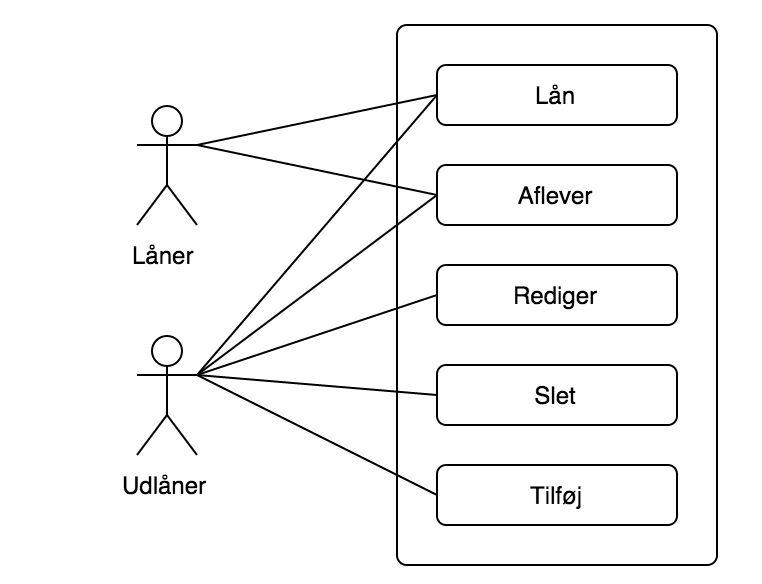
\includegraphics[width=0.8\textwidth]{UseCaseModel}
\end{figure} 

Figur 1 illusterer brugerens råderum. Brugerne af systemet skal have adgang til de samme ting, som en eventuel administrator. Det er altså derfor ikke nødvendigt, at have en administrator. På figuren ses det, at brugeren skal have mulighed for at udlåne, slette, aflevere, redigere og tilføje IT-udstyr, her primært computere. På baggrund af, at vi stadig er i startfasen af kodningen af programmet, så vil det være muligt for kunden at få det ændret til, at der både skal være en 'standardbruger' og en administrator. Det kan betyde, at det kun administratoren, som kan få lov til at tilføje, redigere og slette  computere. ‘Standard' brugeren vil altså kun have mulighed for at lave et udlån, og registrere at en computer er blevet afleveret.
\newpage
\begin{table}[h]
\caption{Use-case 1}
\begin{tabular}{ll}
Scenario name                 & \underline{GammeltUdåningssystem} \\ \hline
Participating actor           & \underline{bob:Låner} \\
instances                     & \underline{alice:Udlåner} \\ \hline
Flow of evnets                & 1. Bob mangler en computer, da hans egen er gået \\& ned. Han henvender sig derfor til Alice for at låne en.
\\& 2. Alice tjekker i arkivet, om der er en ledig \\& computer. Hun finder en.
\\& 3. Alice giver Bob en seddel, som bob skal udfylde: \\& Computer Mærke og model, S/N Tyveri-ID, \\& Låner, Navn, KEA login, Afdeling, Telefon/mobil, \\& Bemærkninger Underskrift, Låners underskrift \\& KEA Servicedesk Sagsnr, Udlånt af, Dato.
\\& 4 Alice henter computeren til Bob og arkiverer
\\& seddelen.
\end{tabular}
\end{table}
Det ses her hvordan det gamle udlånssystem var forældet, og krævede meget unødvendigt arbejde.\\ \\
\begin{table}[h]
\caption{Use-case 2}
\begin{tabular}{ll}
Scenario name                 & \underline{NytUdlåningssystem-Udlån} \\ \hline
Participating actor           & \underline{bob:Låner} \\
instances                     & \underline{alice:Udlåner}\\ \hline
Flow of evnets                & 1. Bob mangler en computer, da hans egen er gået              	\\& ned. Han henvender sig derfor til Alice for at låne en.
\\& 2. Alice tjekker i arkivet, om der er en ledig \\& computer. Hun finder en.
\\& 3. Alice indtaster Bobs ID og skanner computeren.
\\& 4 Alice henter computeren til Bob.
\end{tabular}
\end{table}

Her er samme process beskrevet, blot med brug af det nye udlånssystem. Her er det tydeligt at processen er meget hurtigere og nemmere.
\begin{table}[h]
\caption{Use-case 3}
\begin{tabular}{ll}
Scenario name                 & \underline{NytUdlåningssystem-Aflevering} \\ \hline
Participating actor           & \underline{bob:Låner} \\
instances                     & \underline{alice:Udlåner}\\ \hline
Flow of evnets                & 1. Bob skal aflevere en computer, som han har lånt 
\\& ned. Han henvender sig derfor til Alice for at aflevere den.
\\& 2. Alice indtaster Bobs brugerID og skanner computeren.
\\& Alice arkiverer computeren
\end{tabular}
\end{table}

Til sidst er afleveringen af Bobs computer beskrevet. Som det ses er dette også hurtigt og let.
\newpage
Figur2\\
\centerline{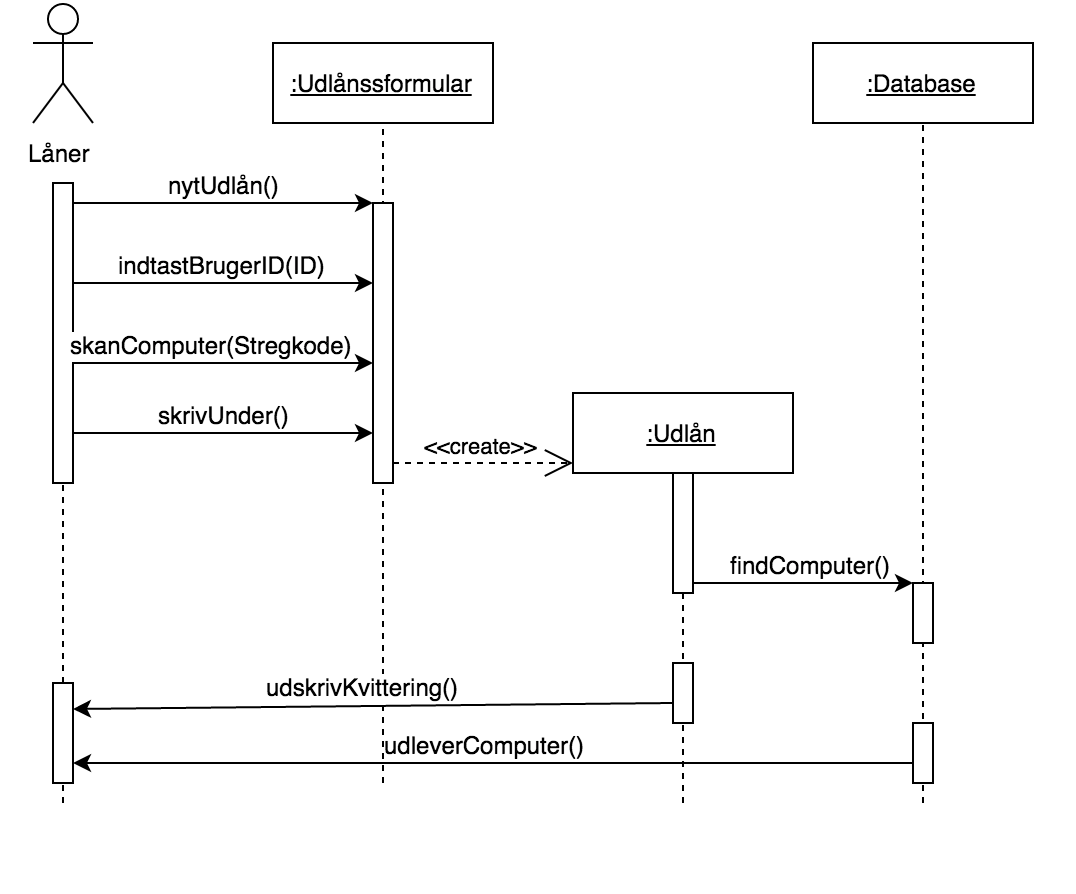
\includegraphics[scale=0.5]{Sekvensdiagram2.png}}
På ovenstående sekvensdiagram vises hvordan det nye udlånssystem kommer til at fungere ved udlån af computer. \\
Figur3\\
\centerline{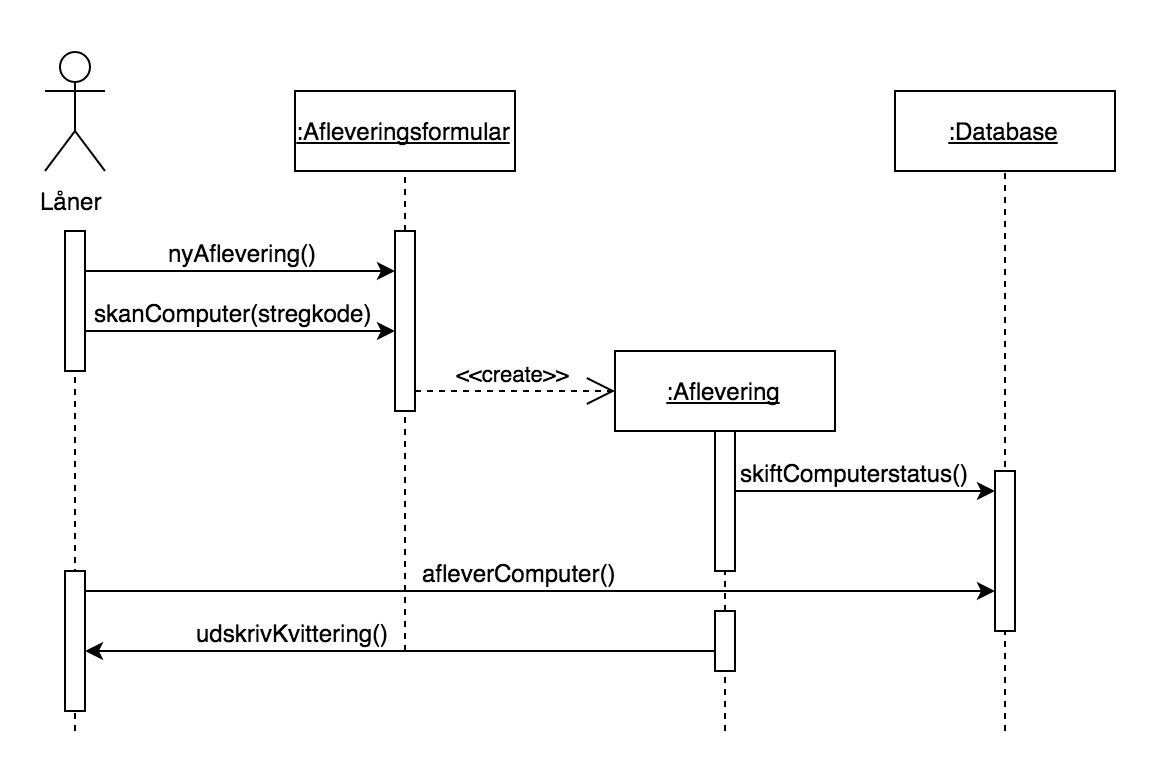
\includegraphics[scale=0.5]{Sekvensdiagram3.png}}
På ovenstående sekvensdiagram vises hvordan det nye udlånssystem kommer til at fungere ved aflevering af computer. Som det ses er processerne for denne og udlån af computer meget ens.
\newpage
\section{Systemdesign}
Systemet er bygget op om en database. Databasens struktur er blevet udviklet, så den kan besvare de spørgsmål vi har til databasen, og så det er nemt for os at udvinde den information vi eller kunden ønsker. Kravene til databasen er, at den skal opbevare data for brugerne, computerne, udlån og historikken for de udlånte computere. Vi lavede først de fire ovennævnte tables. Vi kom frem til den konklusion, at det ikke nemt kunne besvare de simple spørgsmål om hvilke computere var ledige uden, at man skulle slette i tablen for lån. Strukturen er blevet ændret til kun at indholde brugere, computere og lån, hvor historikken findes i lån. Det nuværende design kan også nemt udbygges, hvis kunden har flere krav. \\
Vi har lavet vores backend i Python, hvor vi har lavet et program, som kan hente det data vi har brug for fra databasen. Vores Python program anvender sqlite3 biblioteket. \\
Vi har ikke lavet brugerfladen endnu. Dette vil blive gjort i enten python som et program eller blive en hjemmeside lavet i Django.\\ Grunden til hjemmesiden vil være i Django, er fordi det kan bruge python. Det vil altså være muligt for os at anvende vores python program som backend. Vi har været i kontakt med kunden omkring det skulle være et program eller en hjemmeside. Til dette havde kunden ingen krav, og lader det være op til os. Vi er stadig i processen, hvor vi diskuterer de forskellige fordele og ulemper. En af fordelene ved at lave et python program er, at vi ikke har behov for at lære et nyt sprog, men brugerfladen vil ikke nødvendigvis bliver ligeså køn som hvis det er en hjemmeside. En Fordel ved at lave en hjemmeside er, at der kan laves en pænere brugerflade, men det er et helt nyt som vi skal lære. \\
Vores kunde her derudover os stilt os det krav, at vi skal sikre os at der kan indsættes en underskrift i systemet. Vi har endnu ikke bestemt os for hvordan dette skal gøres. Vi skal enten få underskriften fra en touchpad/mus på en computer, eller koble en tablet til computeren og få brugeren til at skrive sin underskrift på denne. Vi har da tænkt os at opbevare billedet med underskriften i en mappe på et fællesdrev, hvor vi tilknytte de enkelte underskrifter til de der tilhørende udlån. \\
Udestående opgaver, som mangler at bliver lavet: \\
$\bullet$ Front-end. \\
$\bullet$ Implementation af underskrift. \\
$\bullet$ Program som udskriver kvittering, når en computer afleveres.
\section{Program- og systemtest}
Vi har tænkt os at dele program- og systemtest op i to. Vi vil her teste brugervenligheden og om systemet virker som det skal. Vores plan for at teste brugervenligheden er, at vi vil lave Think-Aloud test med vores kunde. Vi vil her observere, hvordan vores kunde færdes i vores system og give vores kunde flere forskellige opgaver som skal løses ved brug af vores system. Vi vil her undervejs notere de gode og dårlige ting ved systemet. Når testen med kunden er færdig, vil vi evaluere testen med kunden, og høre hvad kunden synes om systemet, eller om noget er uhensigtsmæssigt. Think Aloud testen vil blive lavet i forhold til artiklen "Thinking Aloud - User Testing by Molich". \\ \\
Vi vil teste vores system, for at se om det virker som det er tiltænkt. Vi vil altså lave test cases for vores funktioner i python. Vi vil her f.eks. teste, om det er muligt at låne den samme computer ud til to personer på samme tid, om det er muligt at udlåne en fri computer som har været udlånt, men er blevet afleveret. Vi vil altså teste alle de essentielle funktioner, som får systemet til at fungere. Vi vil her teste systemet i forhold til de metoder, som er nævnt i artiklen "Sestoft "Systematic Software Testing" 2008".
\section{Brugergrænseflade og interaktionsdesign}
Ikke implementeret endnu.\\
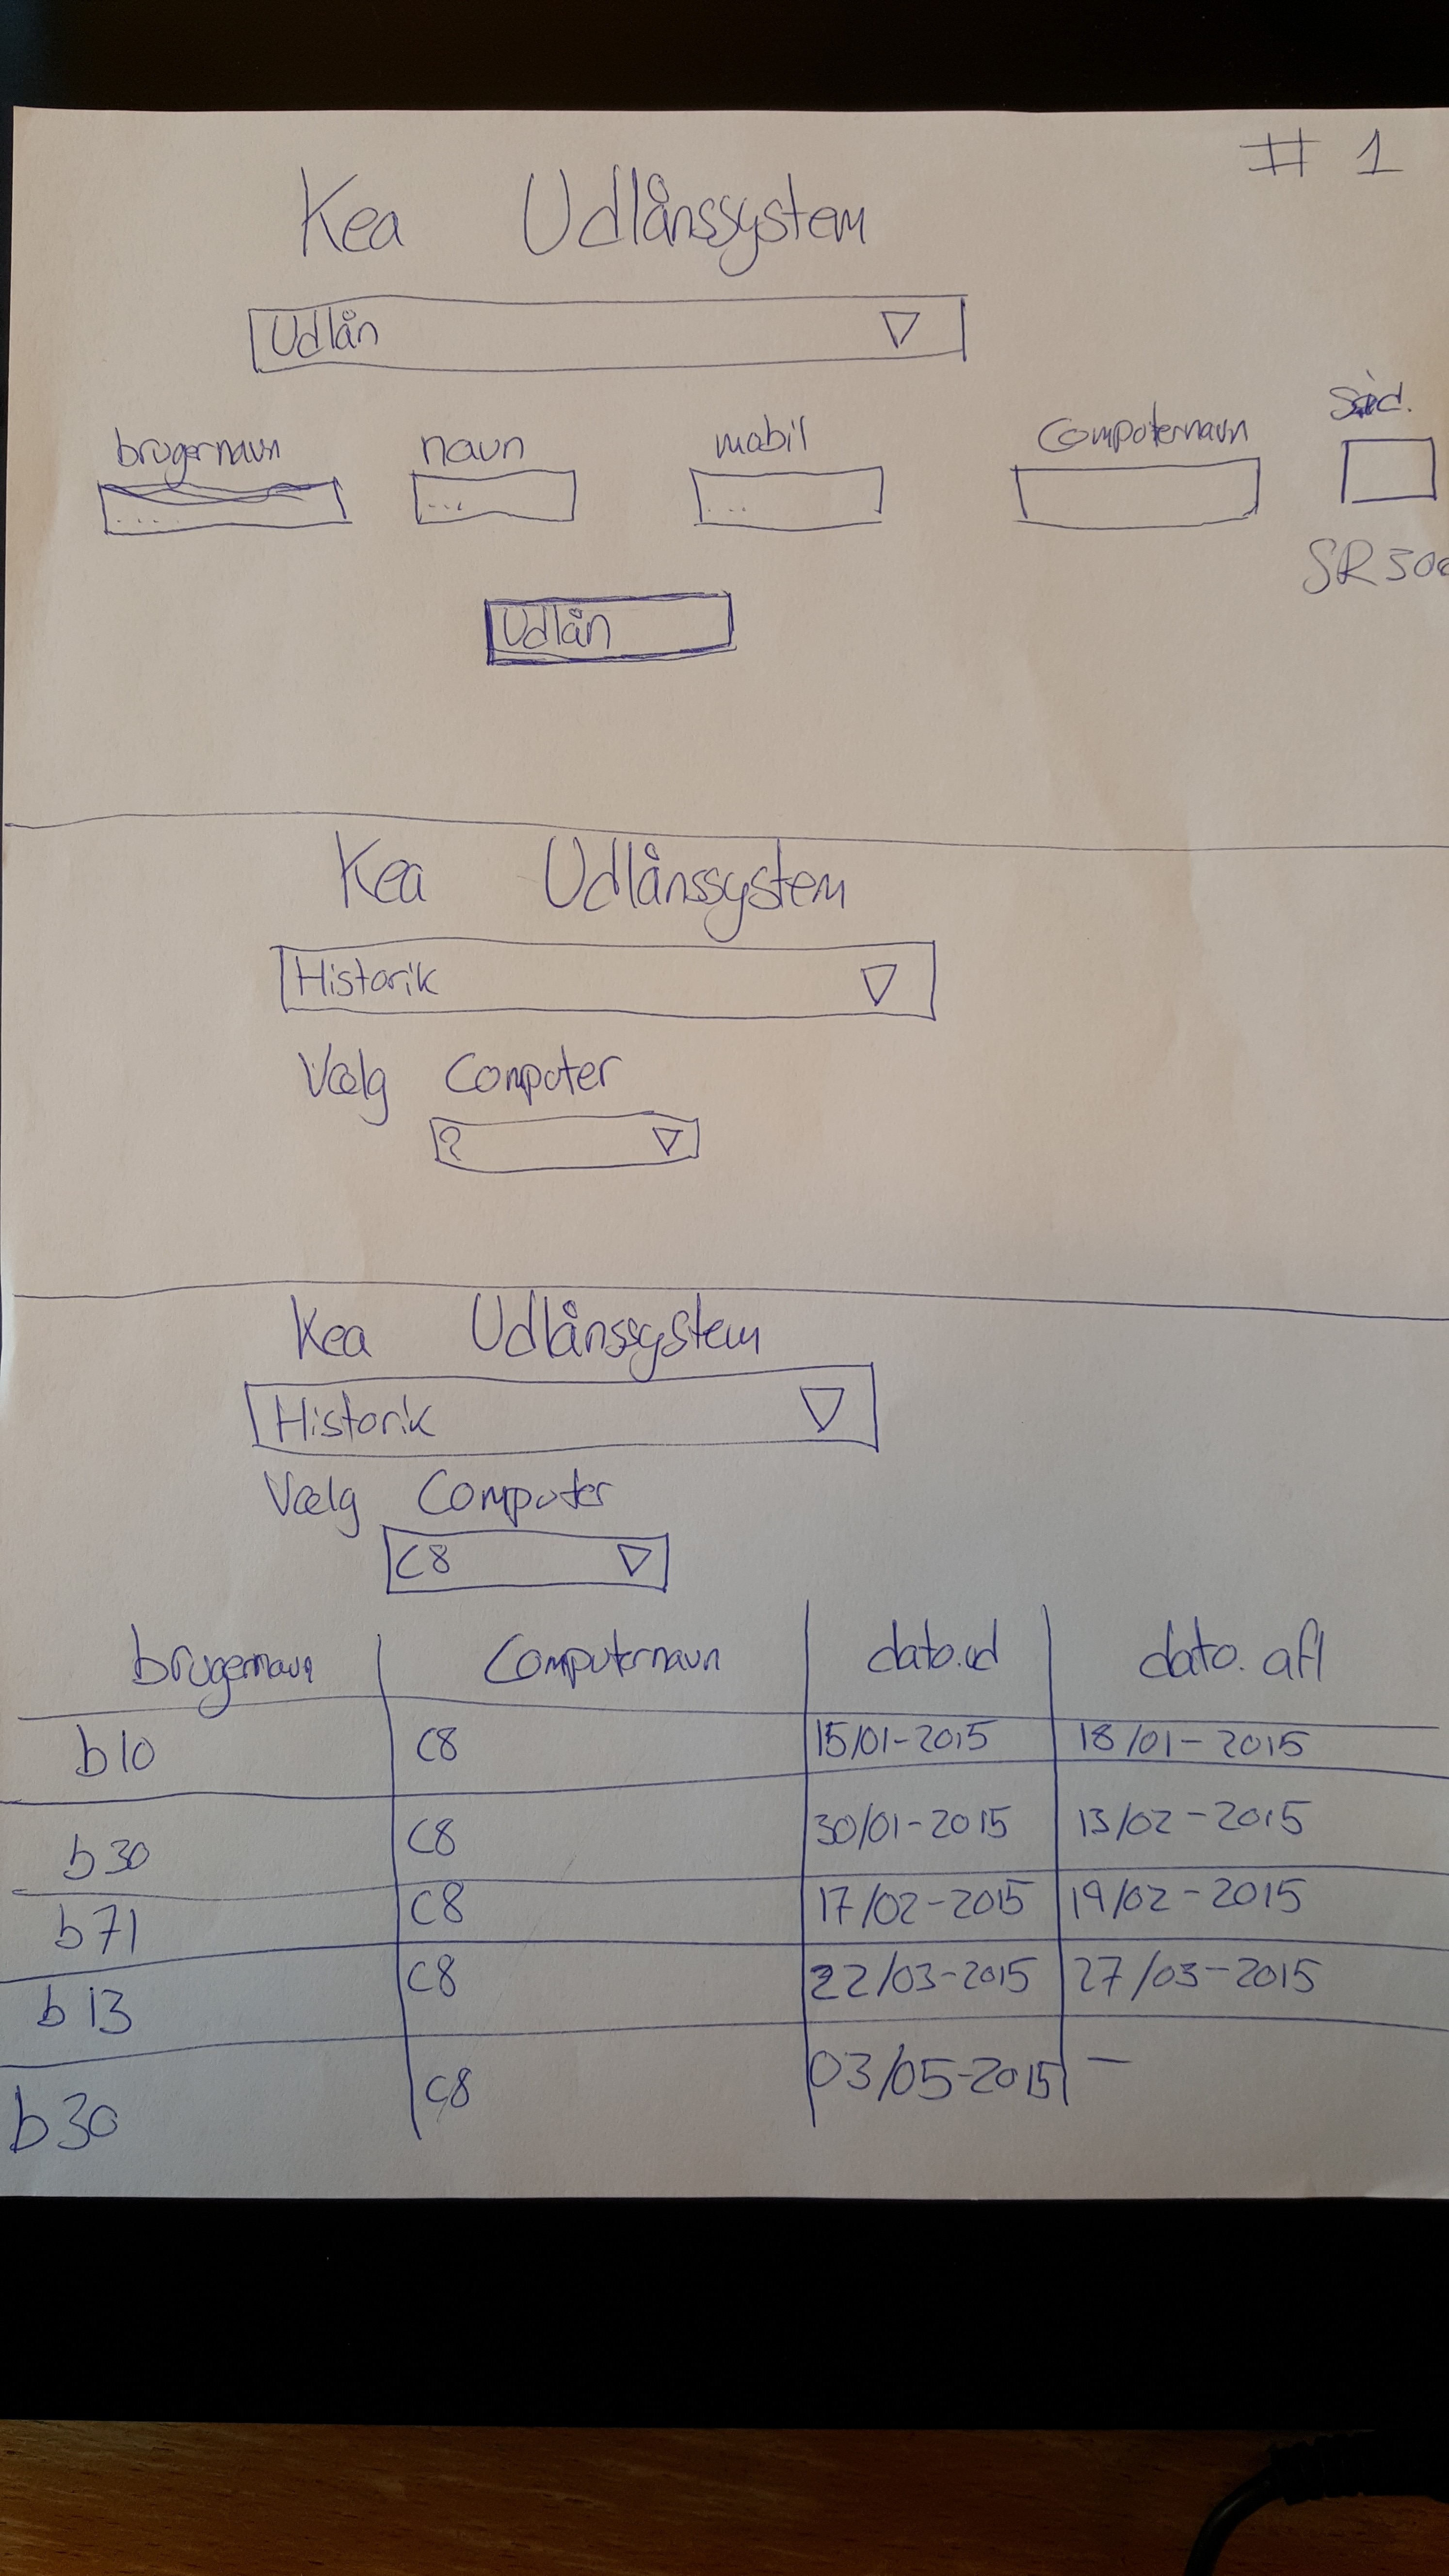
\includegraphics[scale=0.07]{1.jpg}\\
GUI 1\\
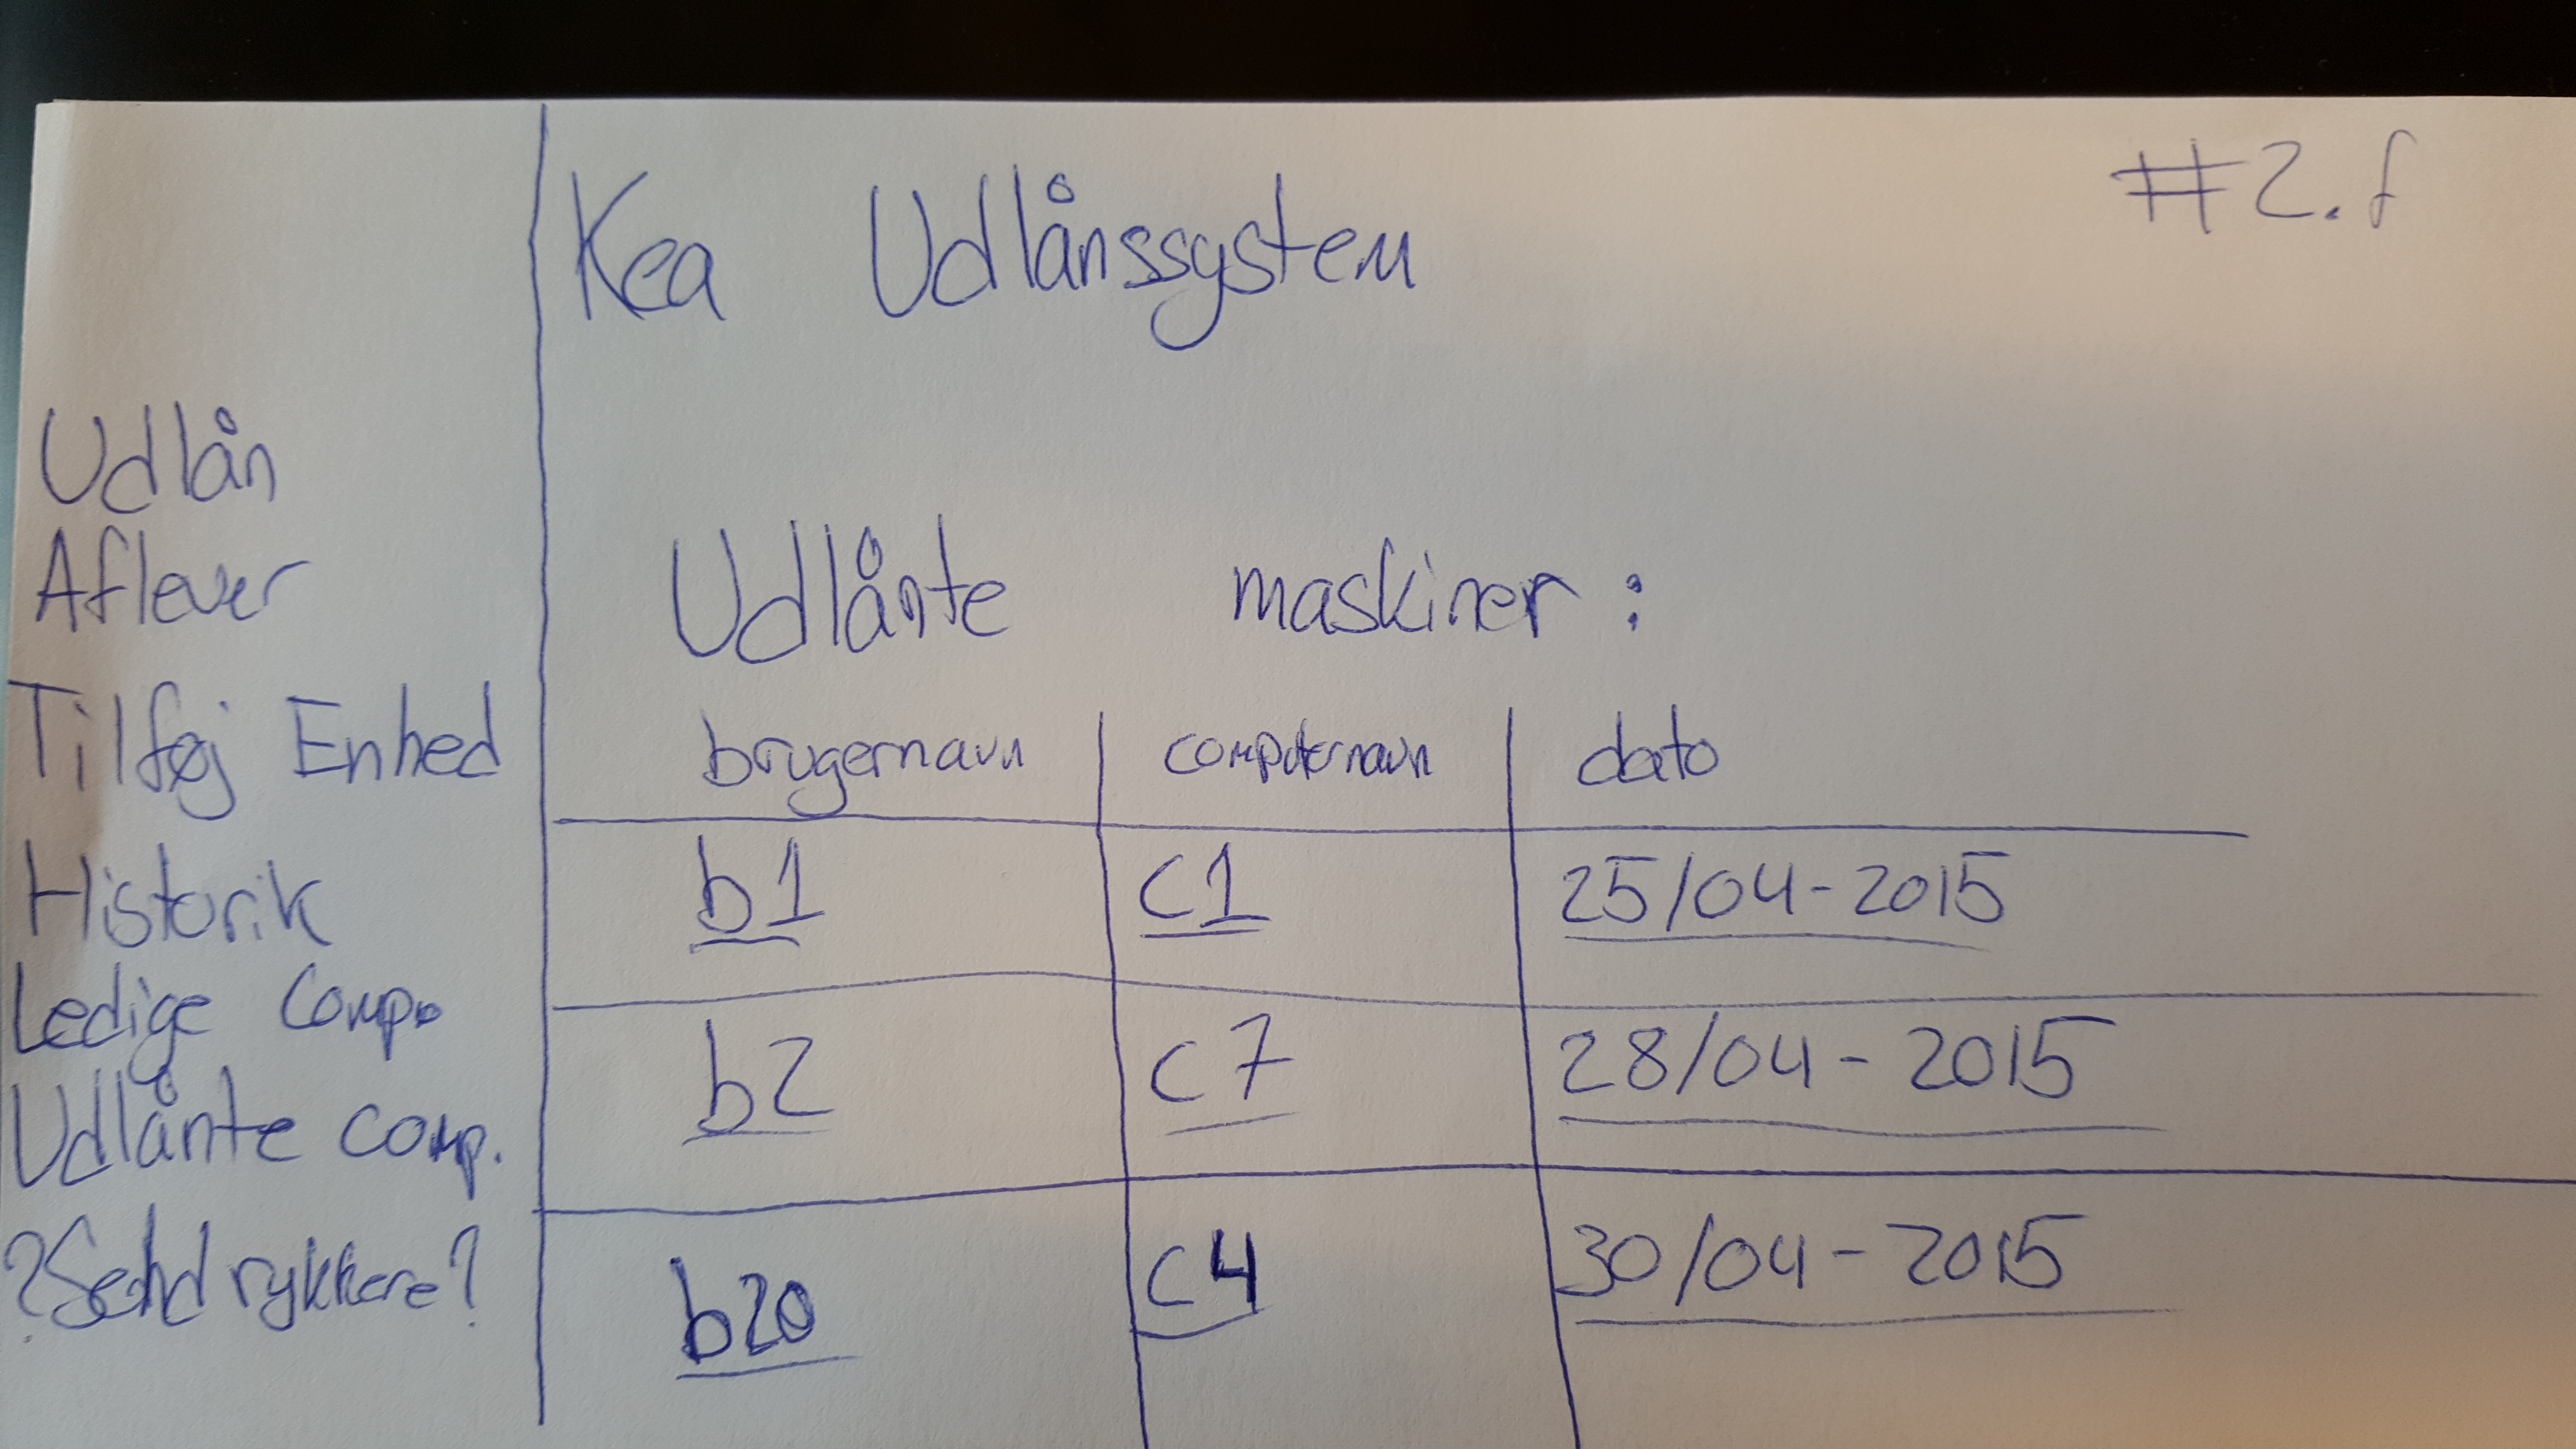
\includegraphics[scale=0.07]{4.jpg}\\
GUI 2\\
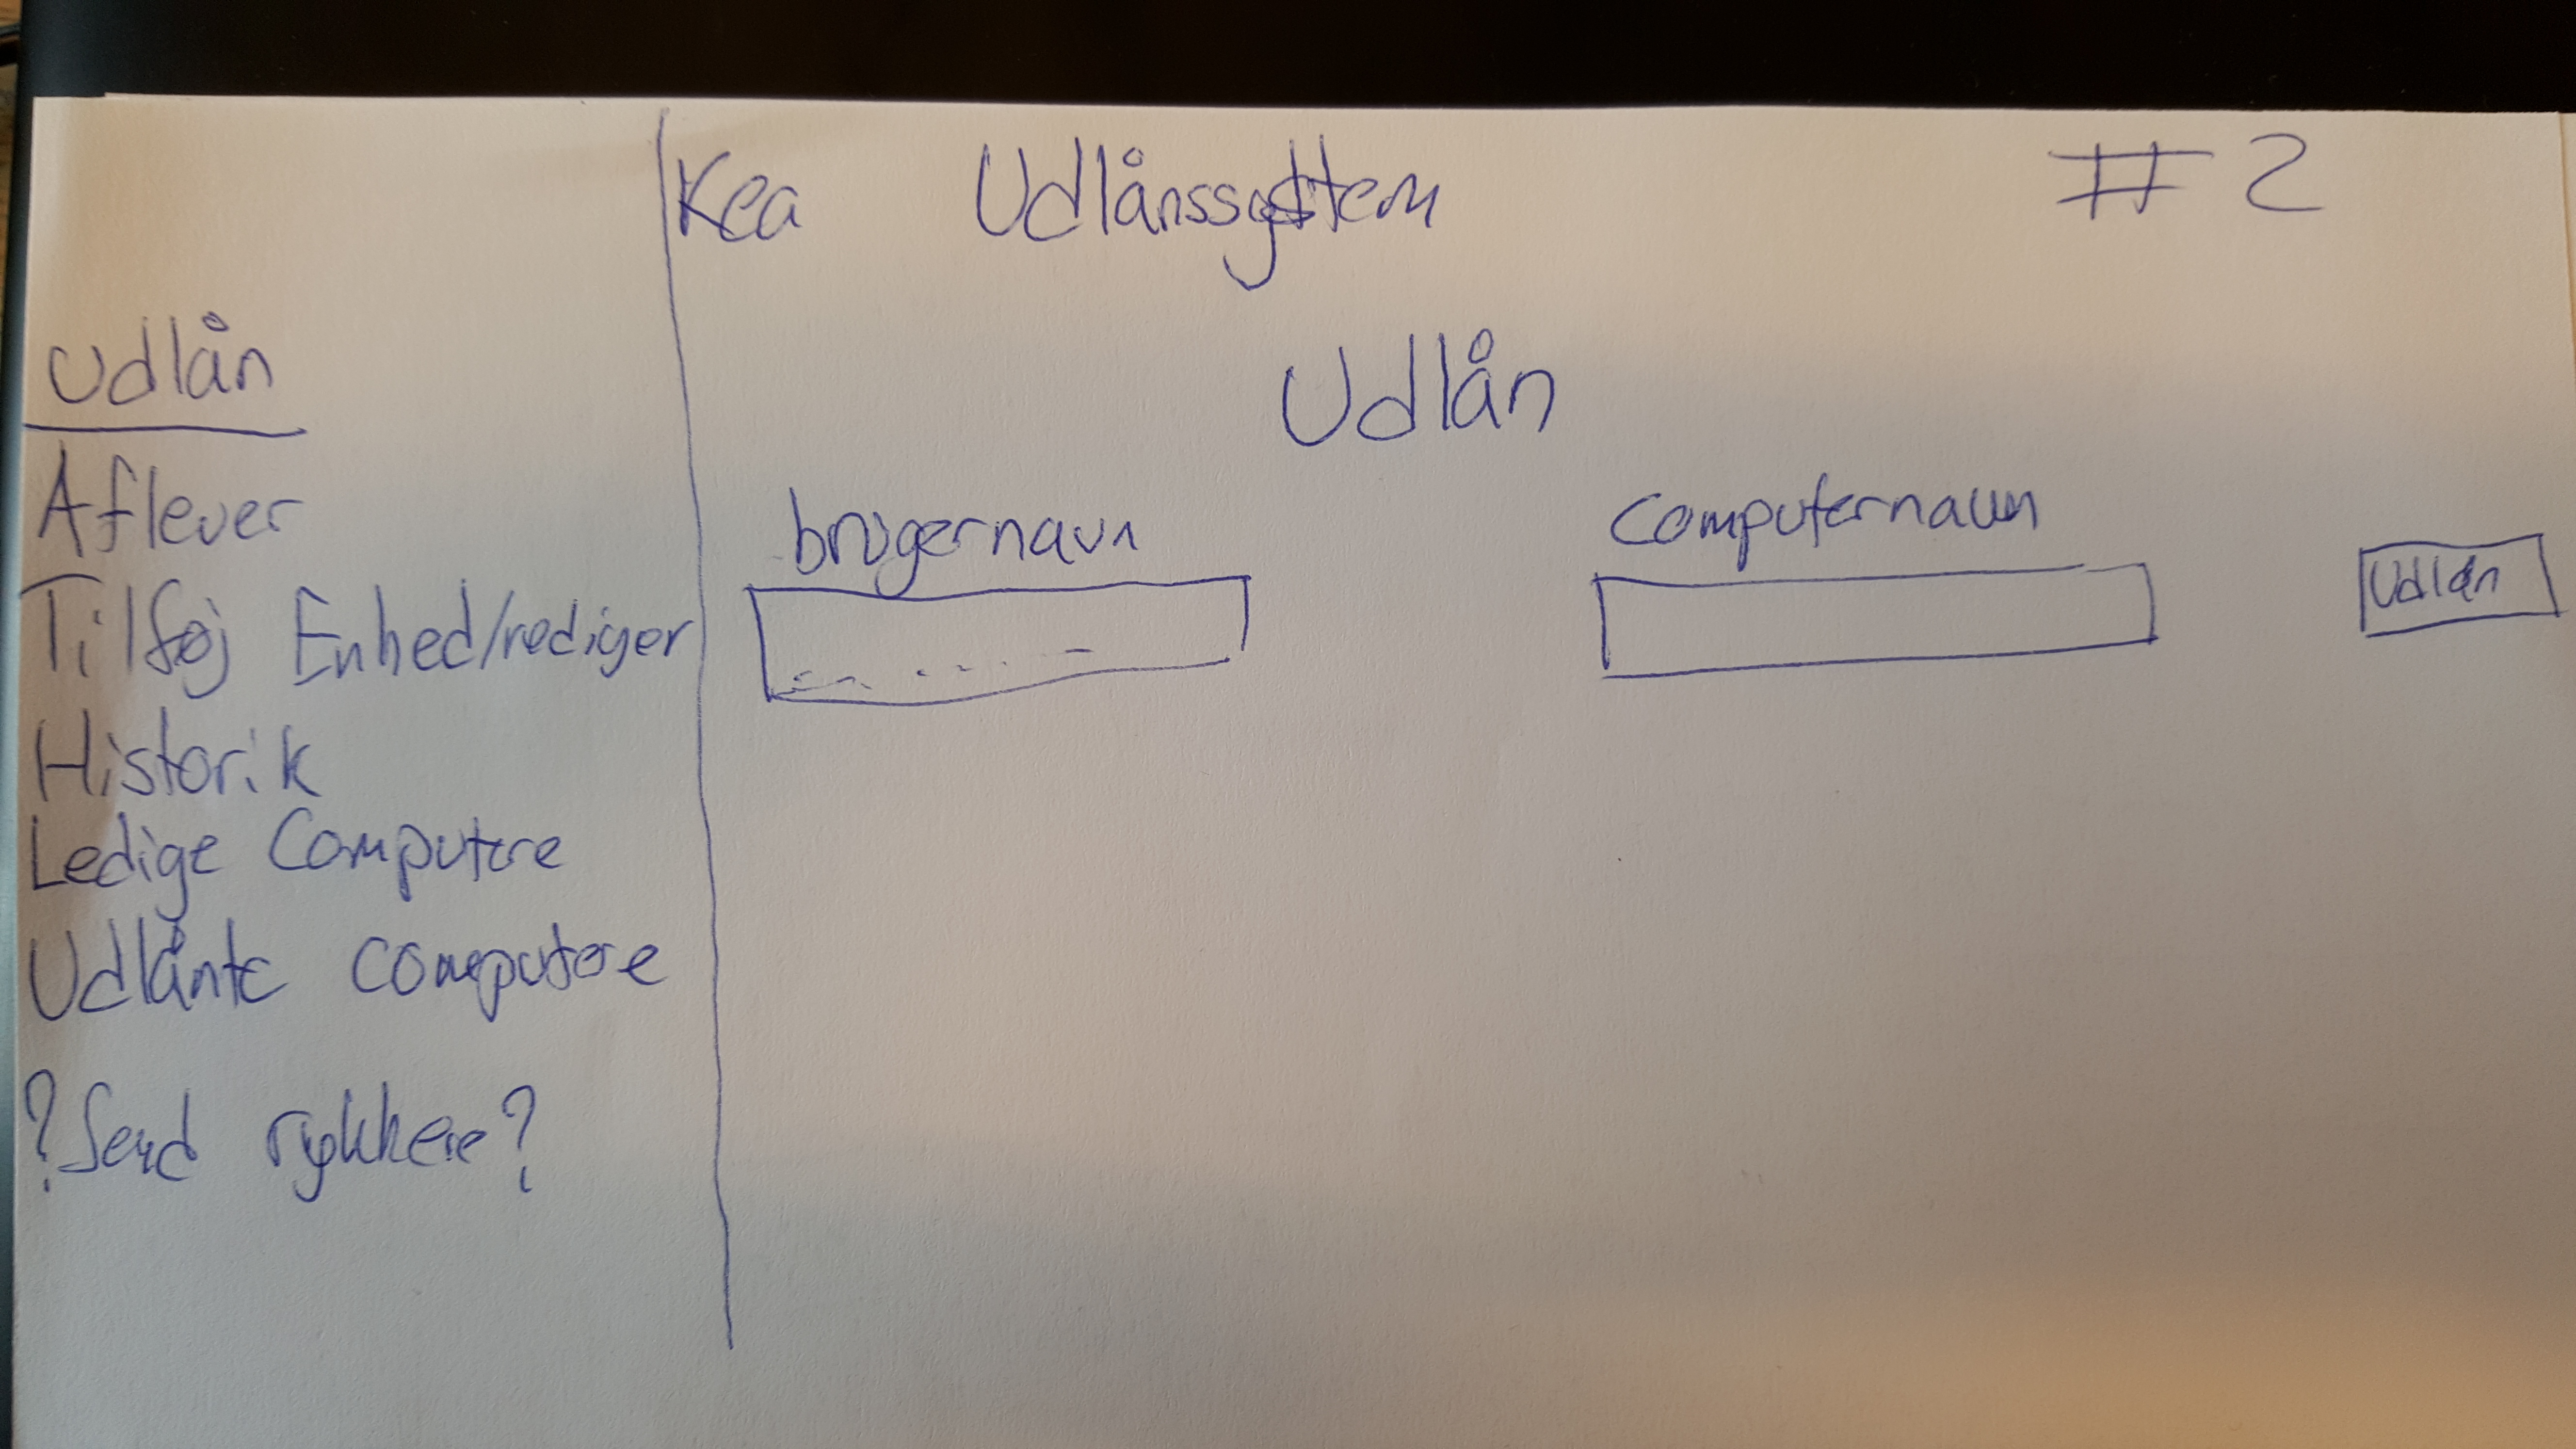
\includegraphics[scale=0.07]{5.jpg}\\
GUI 3\\
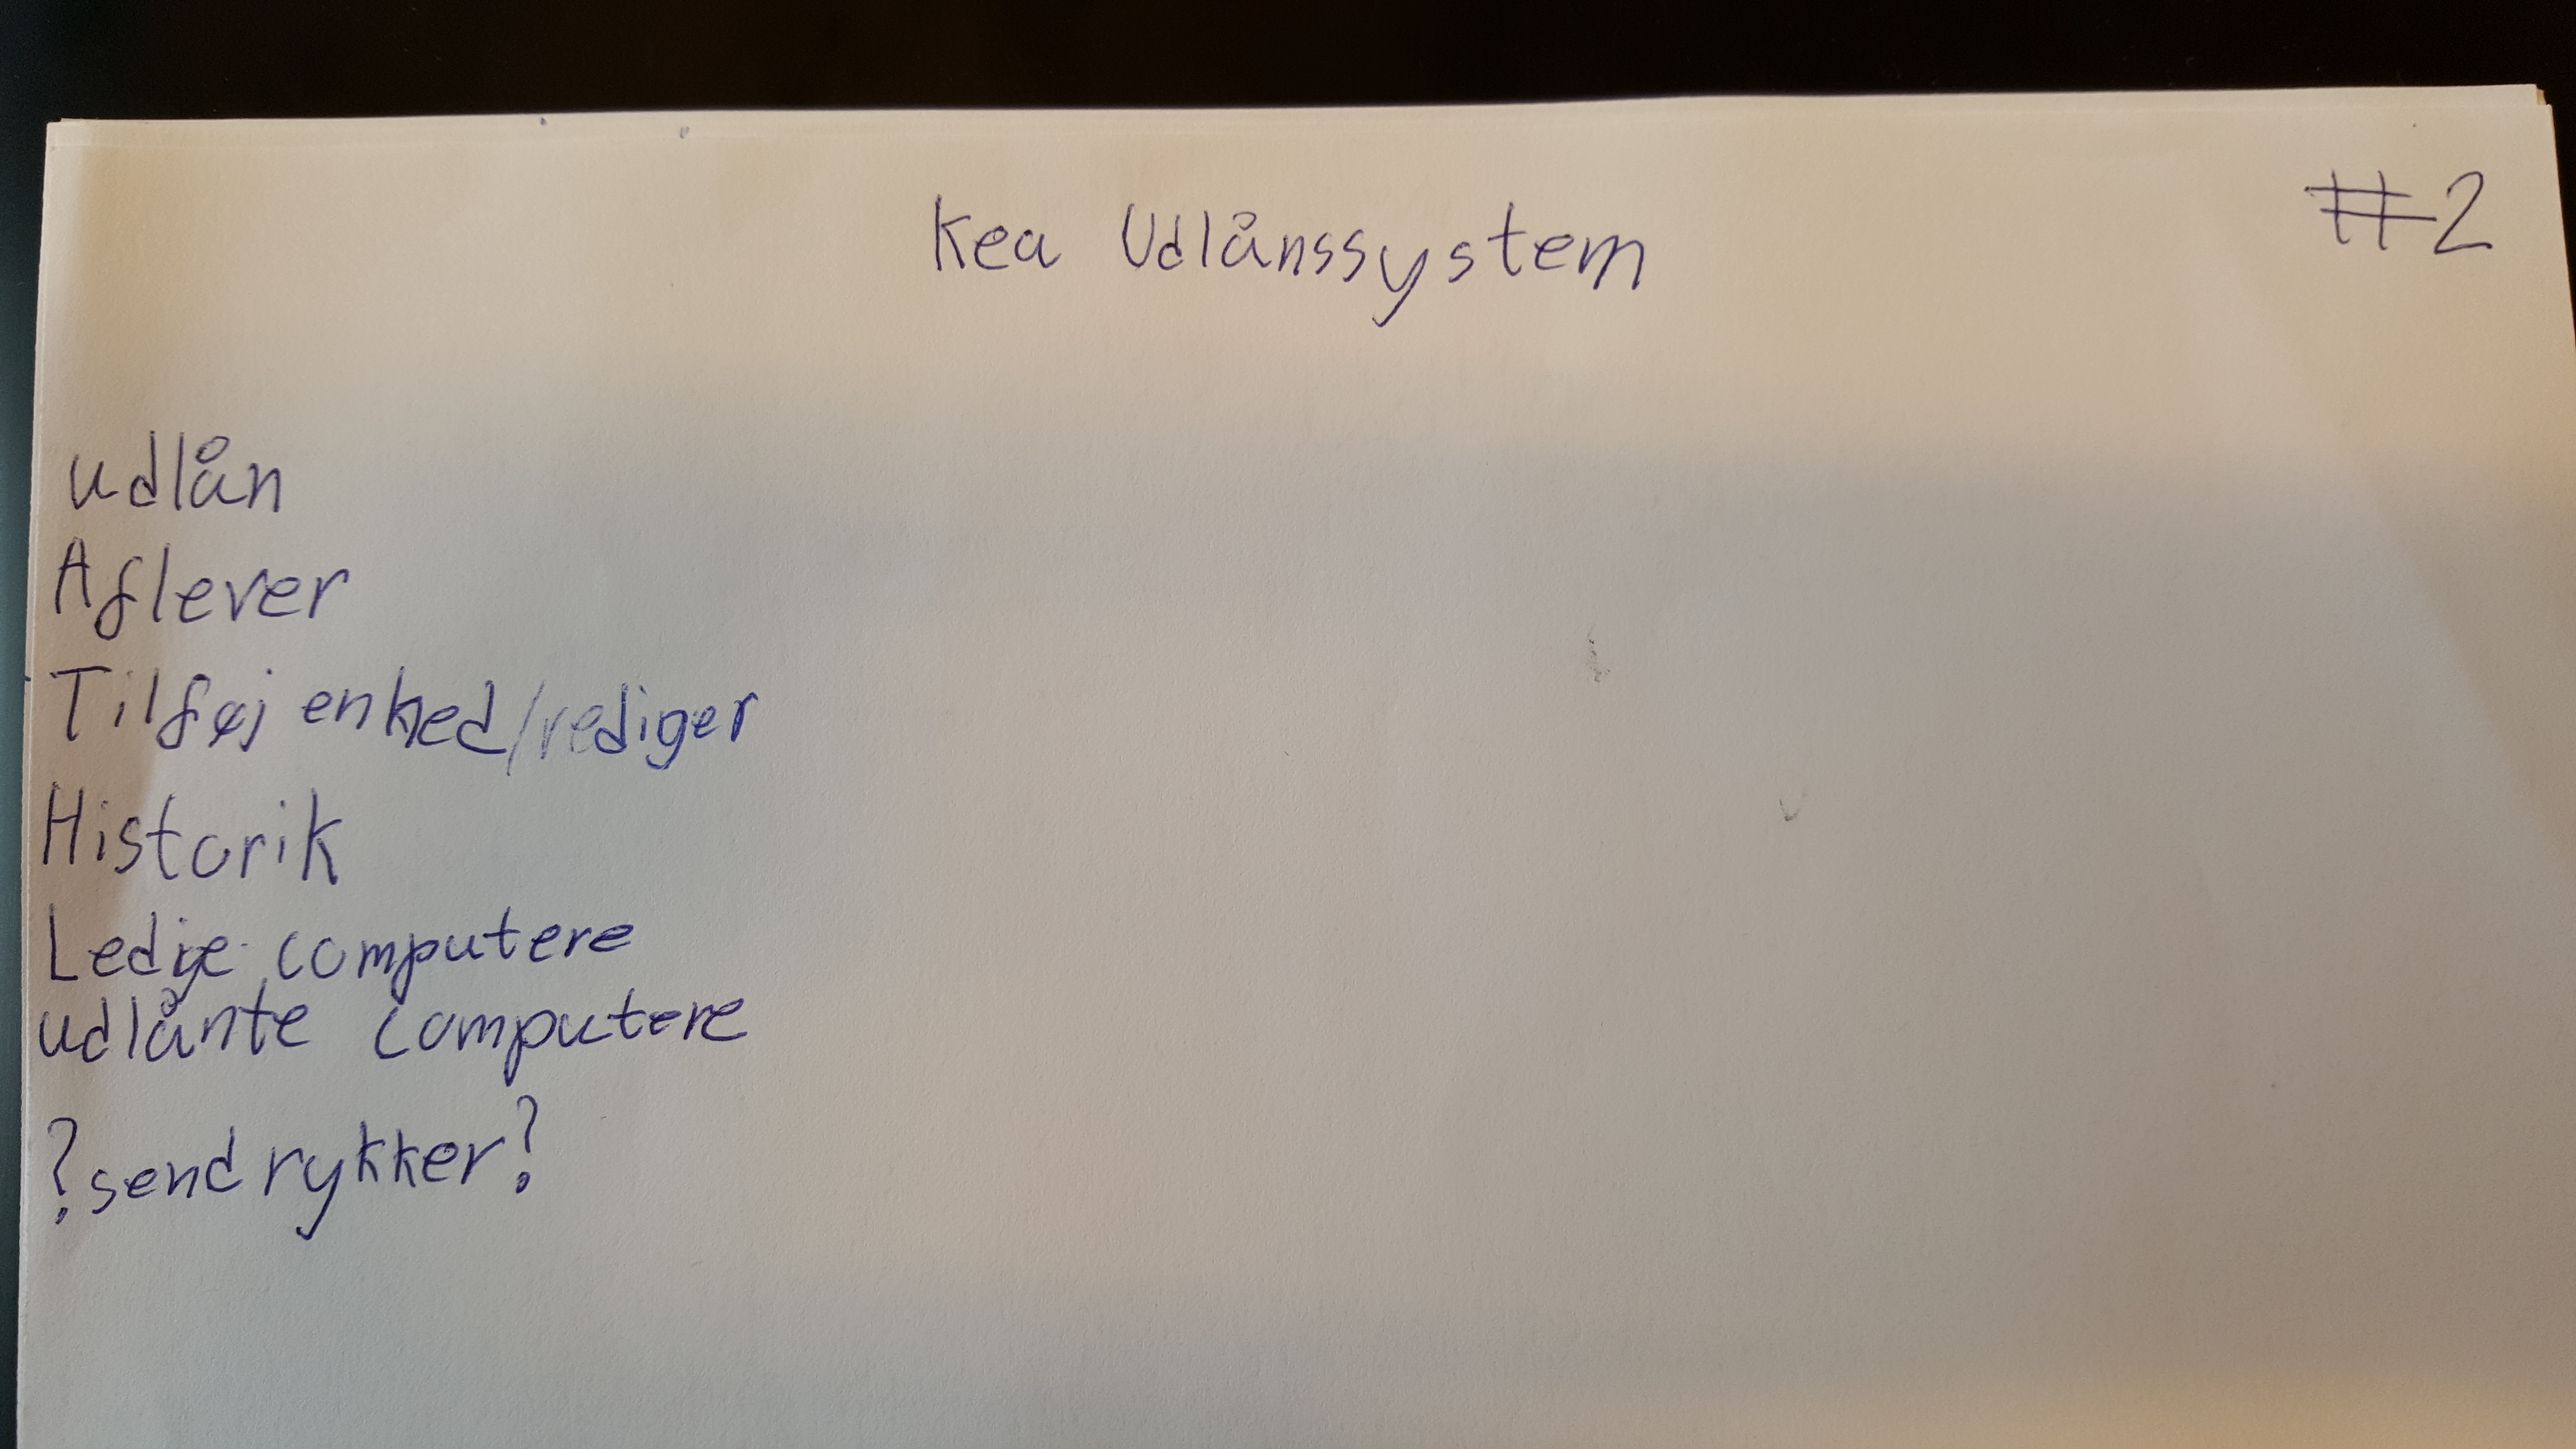
\includegraphics[scale=0.07]{6.jpg}\\
GUI 4\\
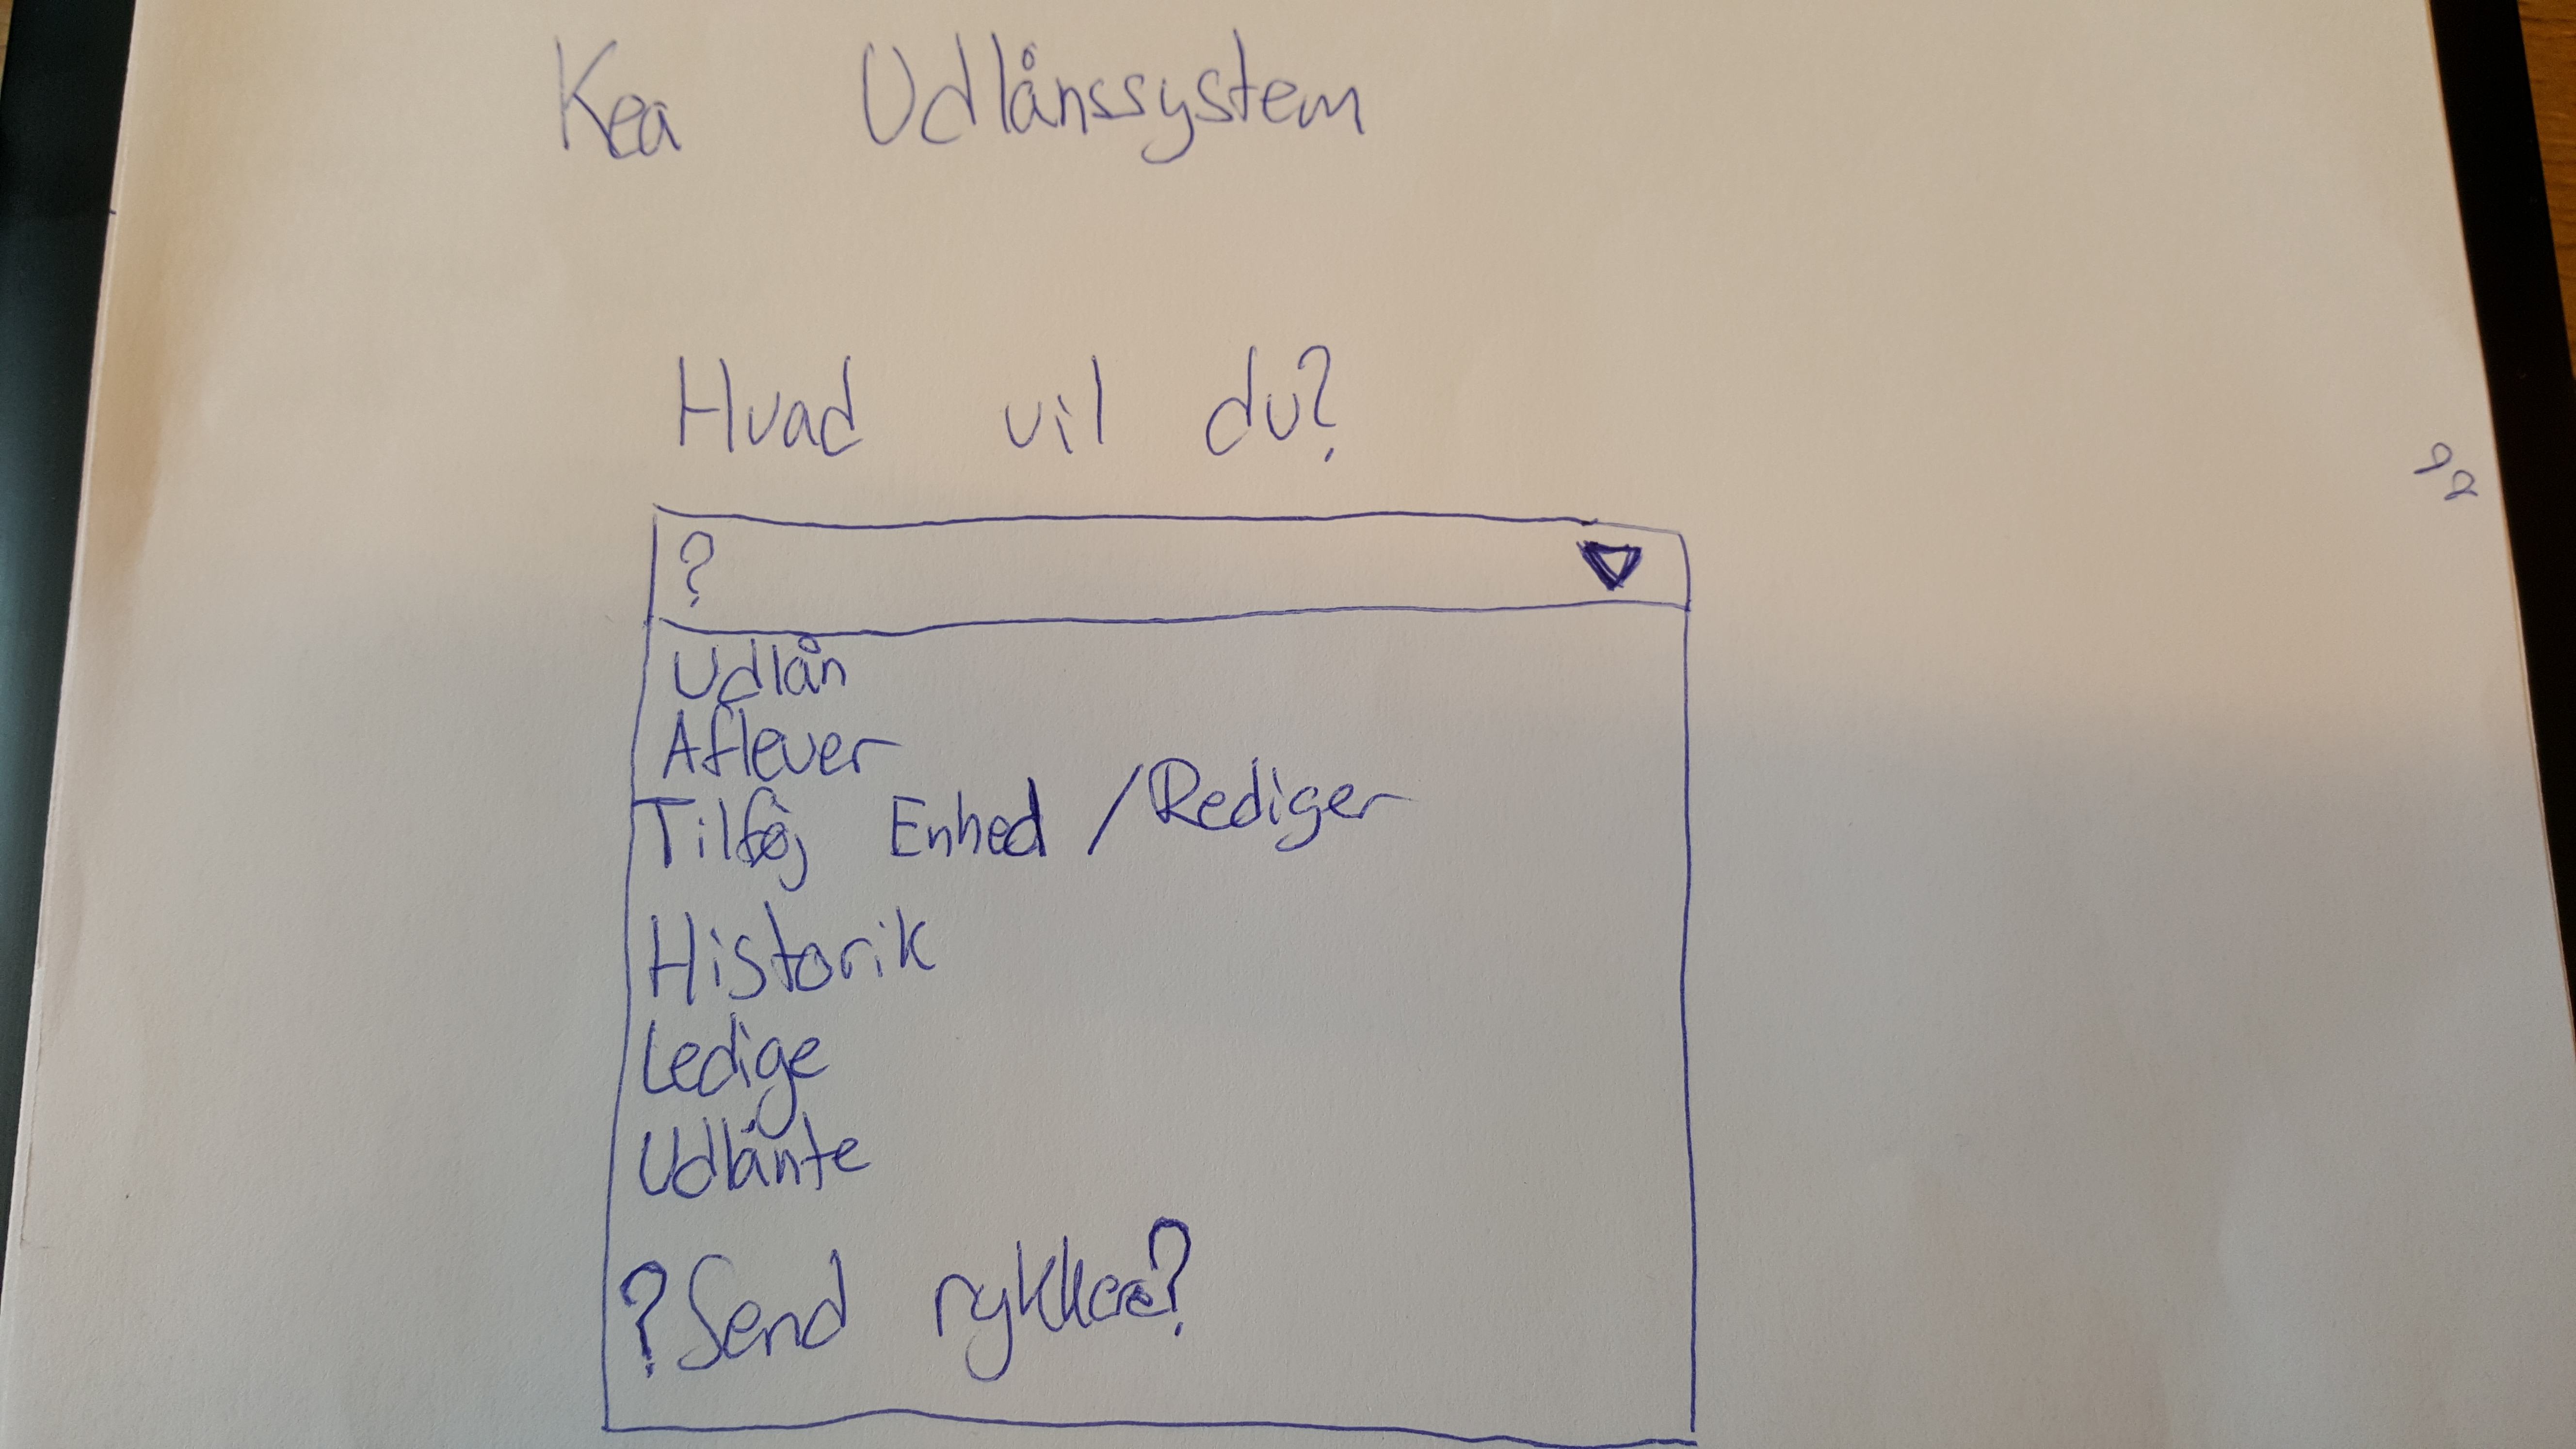
\includegraphics[scale=0.07]{7.jpg}\\
GUI 5\\
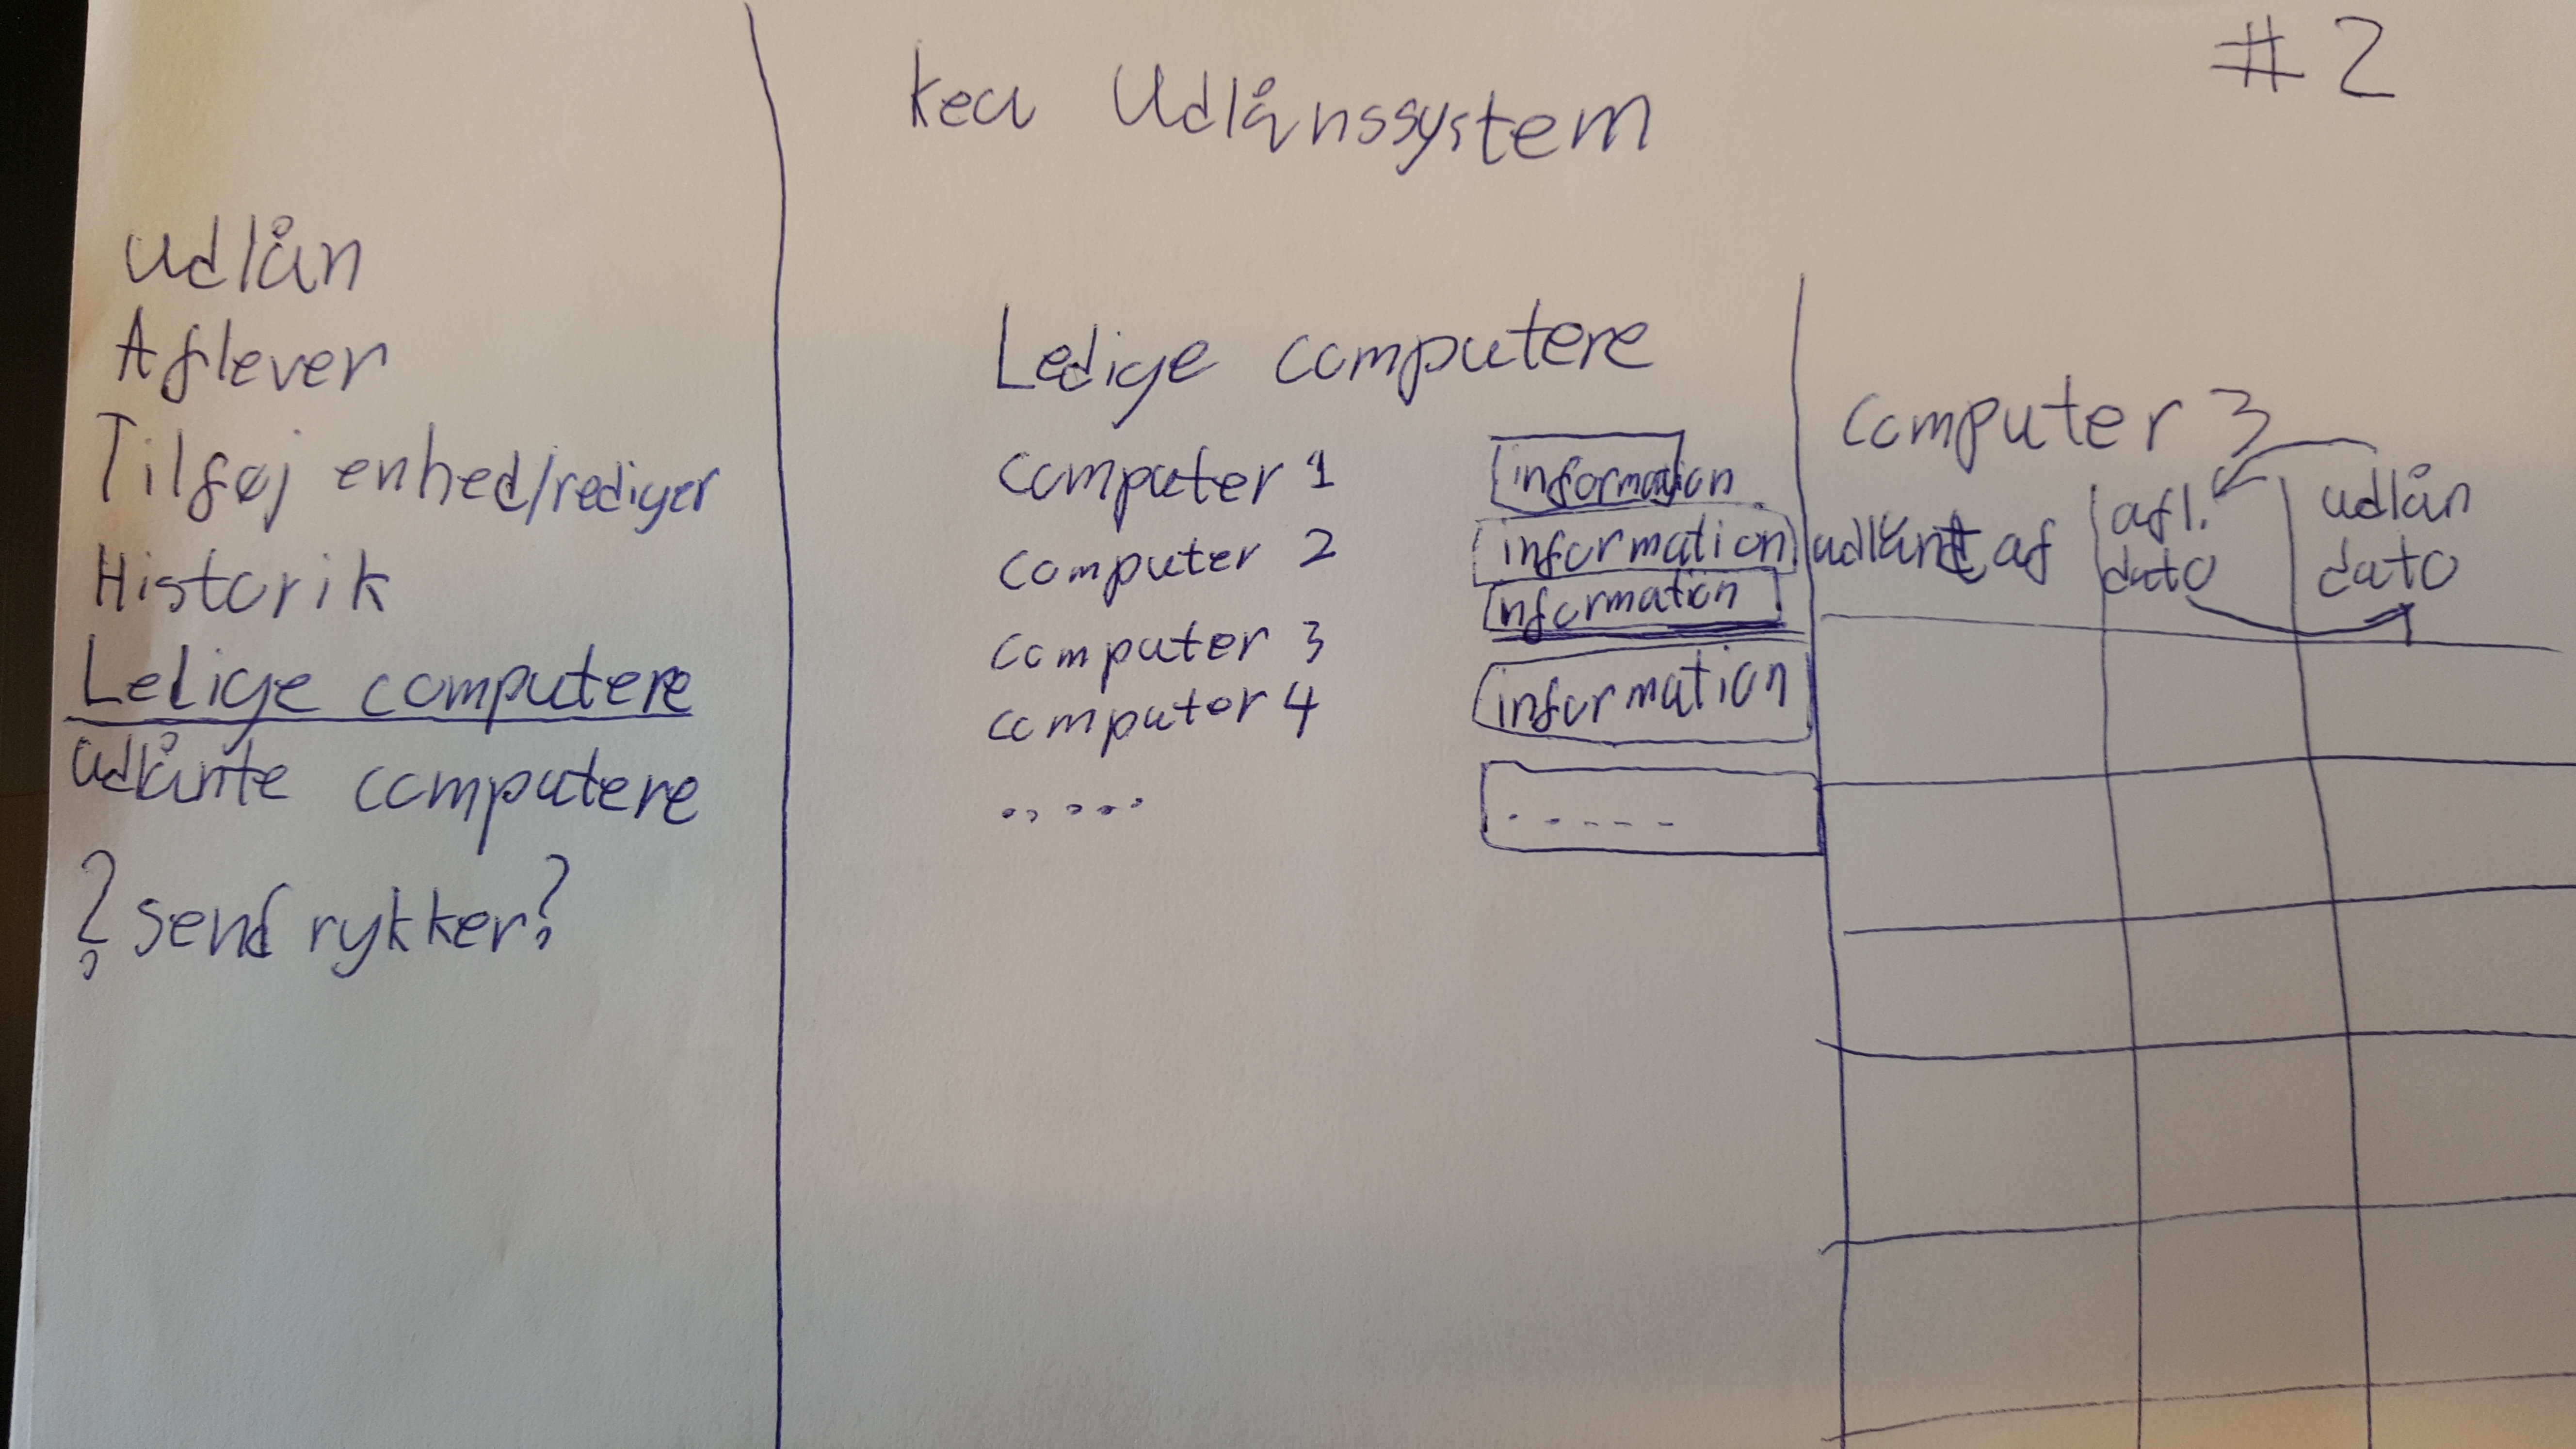
\includegraphics[scale=0.07]{8.jpg}\\
GUI 6\\\\
På de overnstående billeder GUI 1-6 ses de ideer vi har til hvordan det kunne komme til at se ud.\\
Dette er dog stadig kun ide face af hvordan det muligtvis kunne komme til at se ud, derfor har vi en masse forskellige GUI ideer som vi kan se forskellige gode aspekter ved.
\section{Projektsamarbejdet}
Når der ses på samarbejdet mellem gruppen og kunden, ser vi det som værende ikke fyldstgørende. Dette er i den forstand, at der har været nogle uklarheder, som vi først har fået besvaret relativt sent. Det har endnu ikke været muligt for os at etablere et møde, men vi har modtaget en mail som har gjort op for nogle af uklarhederne omkring projektet. Mailen er vores umiddelbare udgangspunkt for projektet.\\
Arbejdet internt i gruppen skrider still og roligt frem. Vi har indtil videre været ramt af eksamener og re-eksamener hvilket har sat tempoet lidt ned.\\
For at effektivisere vores arbejde med projektet, har vi indført to faste dage hver uge, hvor vi vil sidde og udvikle IT-systemet. Dette er for at sikre, at vi kan leve op til vores egne deadlines, og nå at få den krævende viden for at få et virkende program. Vi ønsker her at lave et startmøde i gruppen, når vi mødes, hvor vi uddelegerer arbejde og sikrer os, at vi alle arbejder på relevante felter. Vi vil efter gruppearbejdet opdatere hinanden på hvad og hvor meget der er blevet lavet.\\
Vi mener indtil videre ikke, at vores arbejdsindsats har været god nok, og det er derfor, at vi har valgt at ændre i vores egen møde struktur og indføre to faste dage.
\newpage
\section{Bilag 3 - Timeline}
På nuværende tidspunkt har vores arbejde ikke været på selve programmet endnu men snarere på ideen bag den, så vi vil have en bedre forståelse af hvilket produkt vi skal ende med. Dog er vores egne deadlines sat således:\\
Prototype klar den 03/05/2015 \\
Test af prototype med kunden den 04/05/2015\\
Vores timeline således ud:\\
$\bullet$ Mail modtaget fra kunde 25-03-2015:\\
Den 25. marts modtog vi mail fra kunden om hvad de ønskede sig af programmet. Kunden ønsker at få mere styr på deres proces og få elimineret deres nuværende papirseddel løsning. De ønsker, at systemet automatisk sender rykkere, men samtidig, at de også manuelt kan dette. Kunden vil gerne have, at systemet kan betjenes ved brug af en håndskanner.\\
$\bullet$ Afholdt gruppemøde 21-04-2015:\\
Den 21. april har vi aftalt, at vi ønsker at have den første prototype klar inden den 3. maj. Vi har endvidere aftalt at have to faste dage om ugen, hvor vi vil arbejde på projektet. Dette valg er truffet for at sikre os, at vores egen deadline vil kunne blive overholdt.
\pagebreak
\section{Reviews}
\subsection{A Rational Design Process: How and Why to Fake It}
\textbf{Hovedpunkter}\\
Den rationelle tankegang efterstræbes i artiklen, men ikke den traditionelle form af slagsen som titlen giver udtryk for.
Der henvises til en løbende udviklingsform som der ses indenfor matematikken.
F. eks. bliver et matematikbevis ikke uddybbet på den måde i starten. Det starter med en ide som der derefter arbejdes videre på løbende. Indtil der i sidste ende står et "forhåbentligvis" meget skarpere og kortere bevis end den oprindelige ide var.
Denne form for tankegang kan der draves direkte paralleller til i forhold til programmering.\\
Den rationelle metode vil aldrig kunne blive hundrede procent realiseret indenfor programmeringens verden da usikkerheder og uforudsete problemer ikke kendes på forhånd. Dertil hører mange argumenter som omhandler menneskelige fejl, mangel på specifikke/ændrende krav fra kunde, dele af ældre projekter ville måske kunne kobles på det nye osv.\\
Længere fremme i artiklen kommer det store spørgsmål på, hvorfor denne dokumentation er nødvendig før, under og efter projektet. God dokumentation for det igangværende projekt kan være altafgørende for programmøre der kommer til undervejs i et projekt og fungere som dokumentation af processen så kunde/observatører kan se fremgangen.\\\\
\textbf{Relationer og Tanker}\\
Måden som artiklen beskriver et udviklingsforløb af et projekt ligner meget Scrum metoden.~\cite{Scrum} Især i forhold til den løbende udvikling af produktet. De runs de foregår hvorved løbende prototyper/opgaver skal nåes giver god mening i forhold til denne refleksive/løbende proces af projektet.\\
Kontra bogen~\cite{OOSE} bliver der i denne artikel reflekteret meget over hvad der bliver sagt, vi vil gå så langt som at sige, at teksten er direkte kritisk overfor sig selv. Forstået i den forstand at to sider af en sag bliver taget op. Det ser man for eksempel i artiklen da den fortæller om hvorfor vi skal bruge denne rationelle desgin process, men så alligevel ikke. Bogen er meget "one-sided" i forhold til mange ting, blandt andet denne design process hvor man ikke ser denne reflektion over processen men i stedet fokuserer på at forklare de forskellige metoder.\\
\pagebreak
\subsection{Designing for Usability: Key Principles and What Designers Think}
\textbf{Hovedpunkter}\\
Artiklen sætter fokus på selve bruger-testingen. Der indikeres at for lidt energi bliver lagt i flade udtryk såsom "brugervenlighed", "nemt interface" osv. Mens det der i virkeligheden er brug for er specifik testing af de personer som skal bruge programmet, f. eks. klienten. Artiklen omtaler dette som en meget overset aspekt af udviklingen af et projekt. Der menes at man ville kunne slippe for mange "dumme fejl". Fejl som brugere vil kunne komme ud for som måske ikke så intuitive for en programmør eller designer. Man kan sige, at selve brugervenligheden kan være udsat i større projekter fordi de anses som en udgift i stedet for en nødvendighed.\\
Her starter der en sektion om hvordan man eventuelt ville kunne teste før en eneste linje kode til selve programmet overhovedet er startet.\\\\
\textbf{Relationer og Tanker}\\
Som i den anden artikel~\cite{UseDesign} er der mange antagelser og forudanselser som grundlag for mange af argumenterne. I denne kommer det for eksempel gennem generaliseringen af af hvordan diverse projekter håndteres og hvorledes deres fokuspunkter bliver prioriteret.\\
Artiklen lægger fokus på iterativt design, brugervenlighed og funktonalitet som en vigtig del af et projekts start. Dette spænder godt overens med Scrum metoden~\cite{Scrum} fordi metoden er meget iterativ igennem sine runs hvori man udbygger sit program bid for bid. Undervejs i sådan et forløb får man prototyper/versioner af sit program man kan bruge som:\\
$\bullet$Præsentation til kunder af hvor langt i projektet man er nået og hvilken funkionalitet der er nået/mangler.\\
$\bullet$Løbende versioner som kan testes på brugervenlighed og funktionalitet.\\
$\bullet$Sidst men ikke mindst sikrer man sig at have tidligere versioner af programmet man kan gå tilbage til hvis noget skulle gå galt fra version til version.\\
\pagebreak
\bibliography{bibte}{}
\bibliographystyle{plain}

\end{document}
